\Chapter{REVUE DE LITTÉRATURE}\label{sec:RevLitt}
Cette section aura pour but de dresser l'état des connaissances sur les politiques de stationnement, l'estimation de la capacité de stationnement, les outils d'analyse d'images satellites utilisés pour la détection automatique d'objets, les coûts associés à la provision du stationnement et les méthodes d'estimations pour les stationnements en structure.

\section{Typologie de stationnement}\label{sec:typologie_stationnement}
  \textcite{Morency:StationnementDans:2017} détaillent une typologie de stationnement pour le stationnement hors rue et sur rue pour la région métropolitaine de Montréal montrés aux figures \ref{fig:Typo_Stat_hors_rue} et \ref{fig:Typo_Stat_sur_rue}
  \begin{figure}[ht]
      \centering
      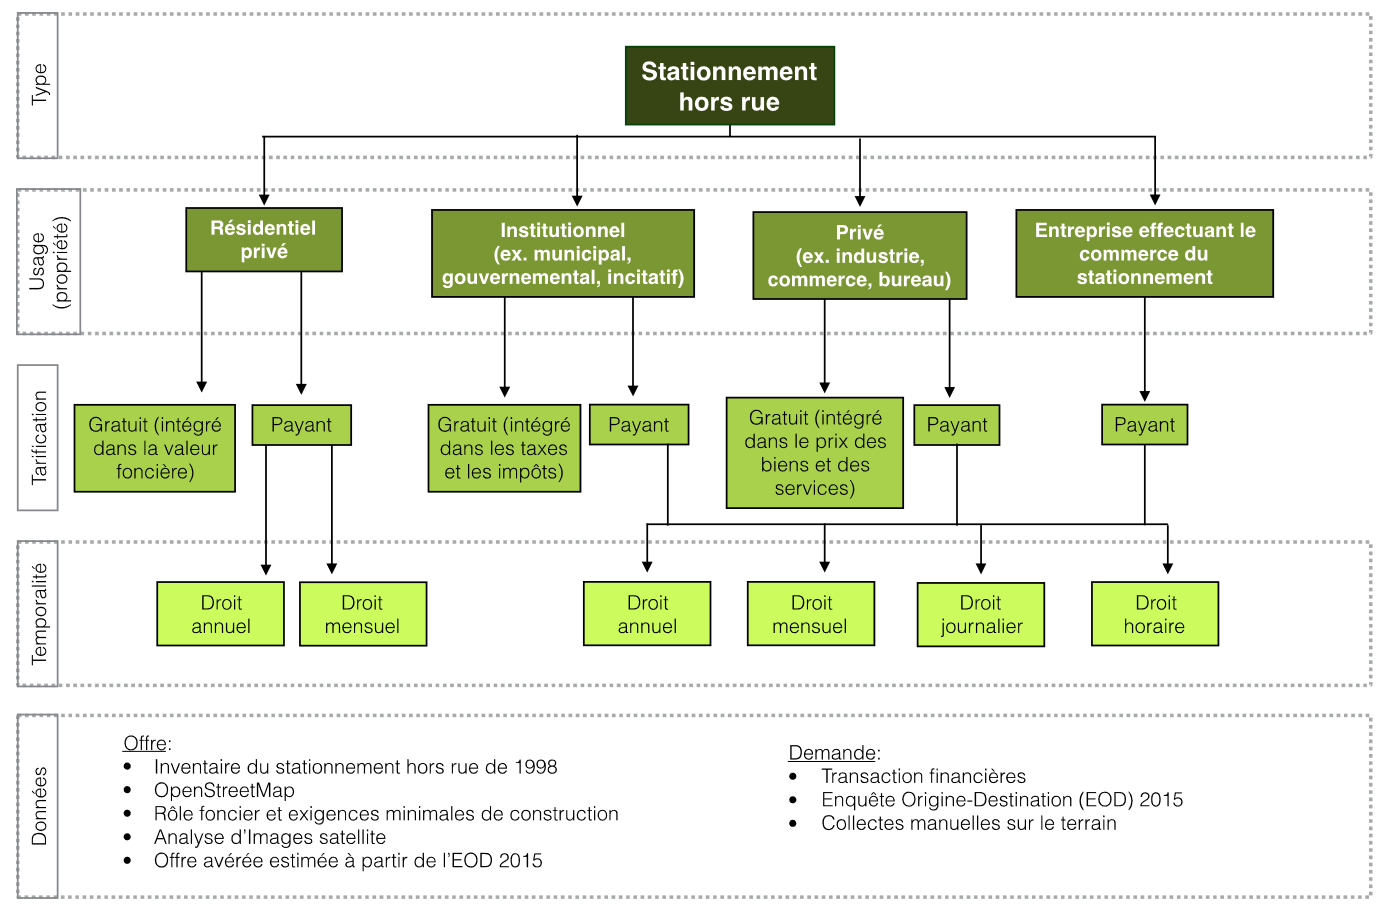
\includegraphics[width=1.0\textwidth]{images/Typologie_Stationnement_hors_rue.png}
      \caption{Typologie de stationnement hors rue. \hl{vérifier droits auteurs} Source: \cite{Morency:StationnementDans:2017}}
      \label{fig:Typo_Stat_hors_rue}
  \end{figure}
  \begin{figure}[ht]
      \centering
      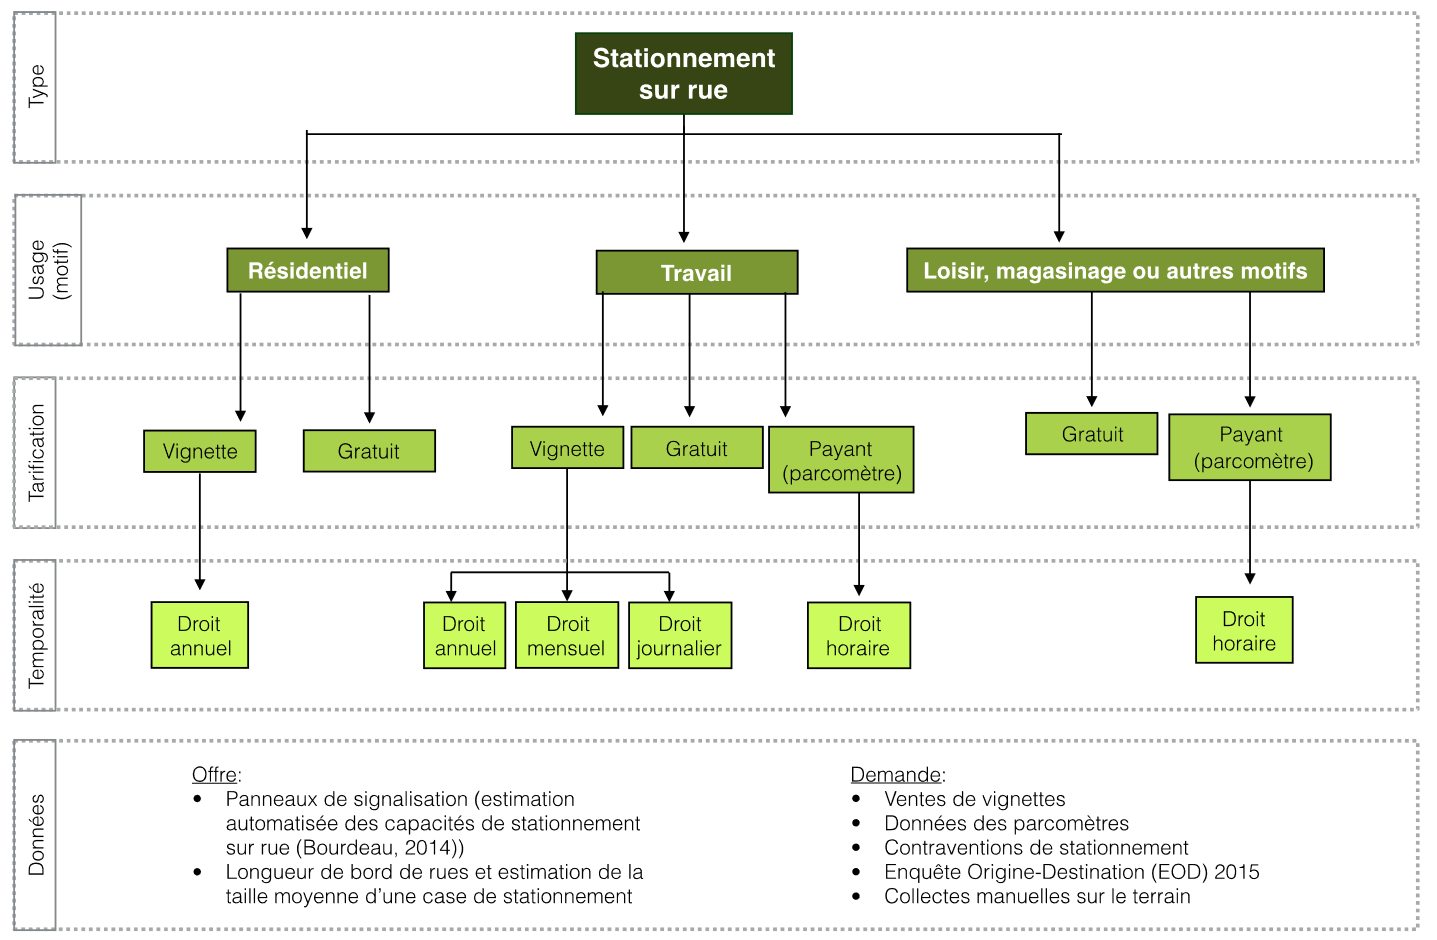
\includegraphics[width=1.0\textwidth]{images/Typologie_Stationnement_sur_rue.png}
      \caption{Typologie de stationnement sur rue. \hl{vérifier droits auteurs} Source: \cite{Morency:StationnementDans:2017}}
      \label{fig:Typo_Stat_sur_rue}
  \end{figure}
  Il est important de noter qu'il n'existe pas à la connaissance de l'auteur un inventaire tel que celui complété par le ministère des Transports pour la ville de Montréal \parencite{ConsortiumCIMA+-DanielArbouretassocies:InventaireEspaces:1998}. D'autre part, cet inventaire n'est pas mis à jour régulièrement et n'est donc pas particulièrement utile pour la mise à jour de plans de transports.